\begin{frame}
\frametitle{Method}
\framesubtitle{Adding Conditioning Input}
\begin{figure}
    \centering
    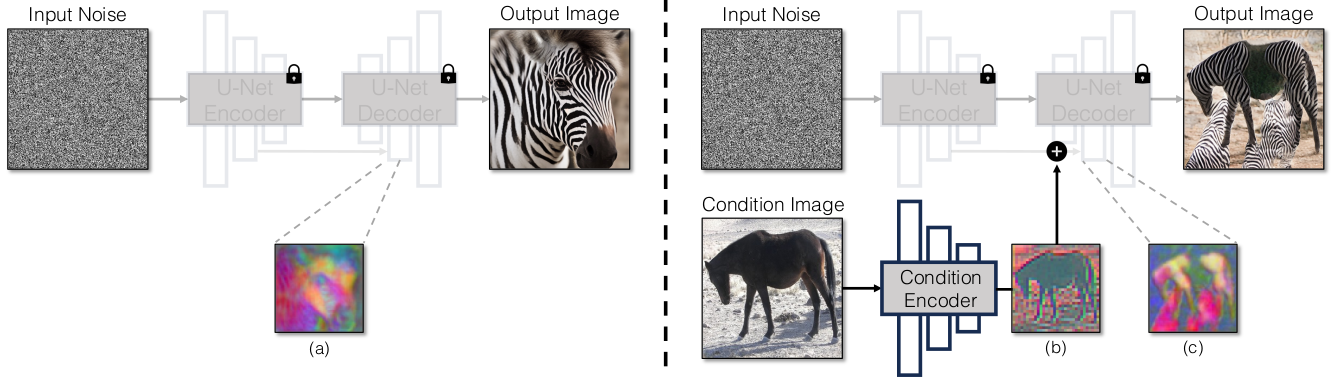
\includegraphics[width=1\linewidth]{images/Bildschirmfoto vom 2024-04-14 10-57-39.png}
    \caption{Conflicts between noise and conditional input}
\end{figure}
\end{frame}

% ---------- Preserving Input Details ----------
\begin{frame}
\frametitle{Method}
\framesubtitle{Preserving Input Details}
\begin{figure}
    \centering
    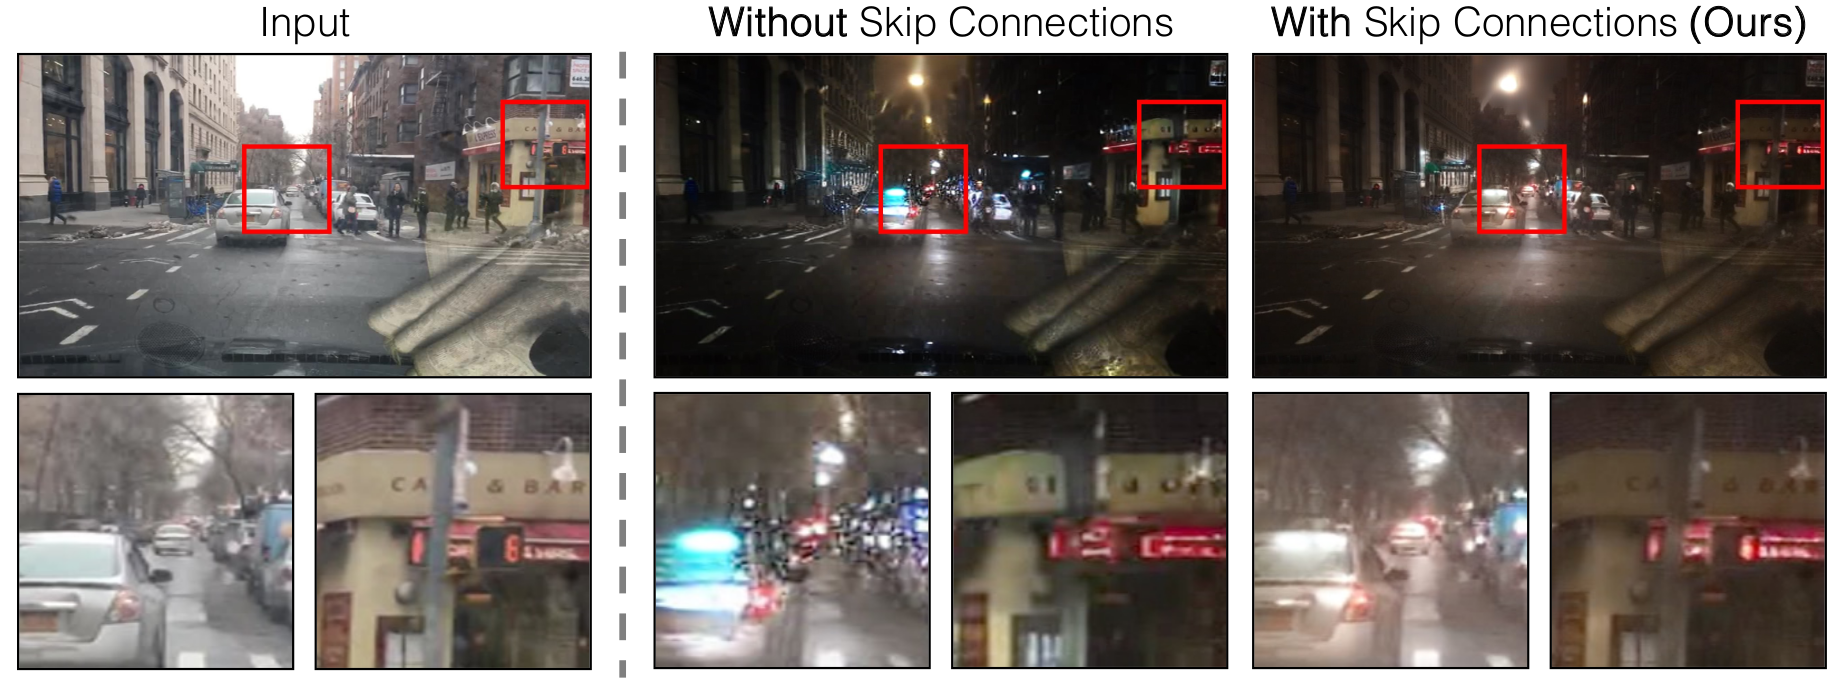
\includegraphics[width=0.9\linewidth]{images/Bildschirmfoto vom 2024-04-14 11-06-40.png}
    \caption{Skip Connections help retain details}
\end{figure}
\end{frame}

% ---------- Preserving Input Details ----------
\begin{frame}
\frametitle{Method}
\framesubtitle{Preserving Input Details}
\begin{figure}
    \centering
    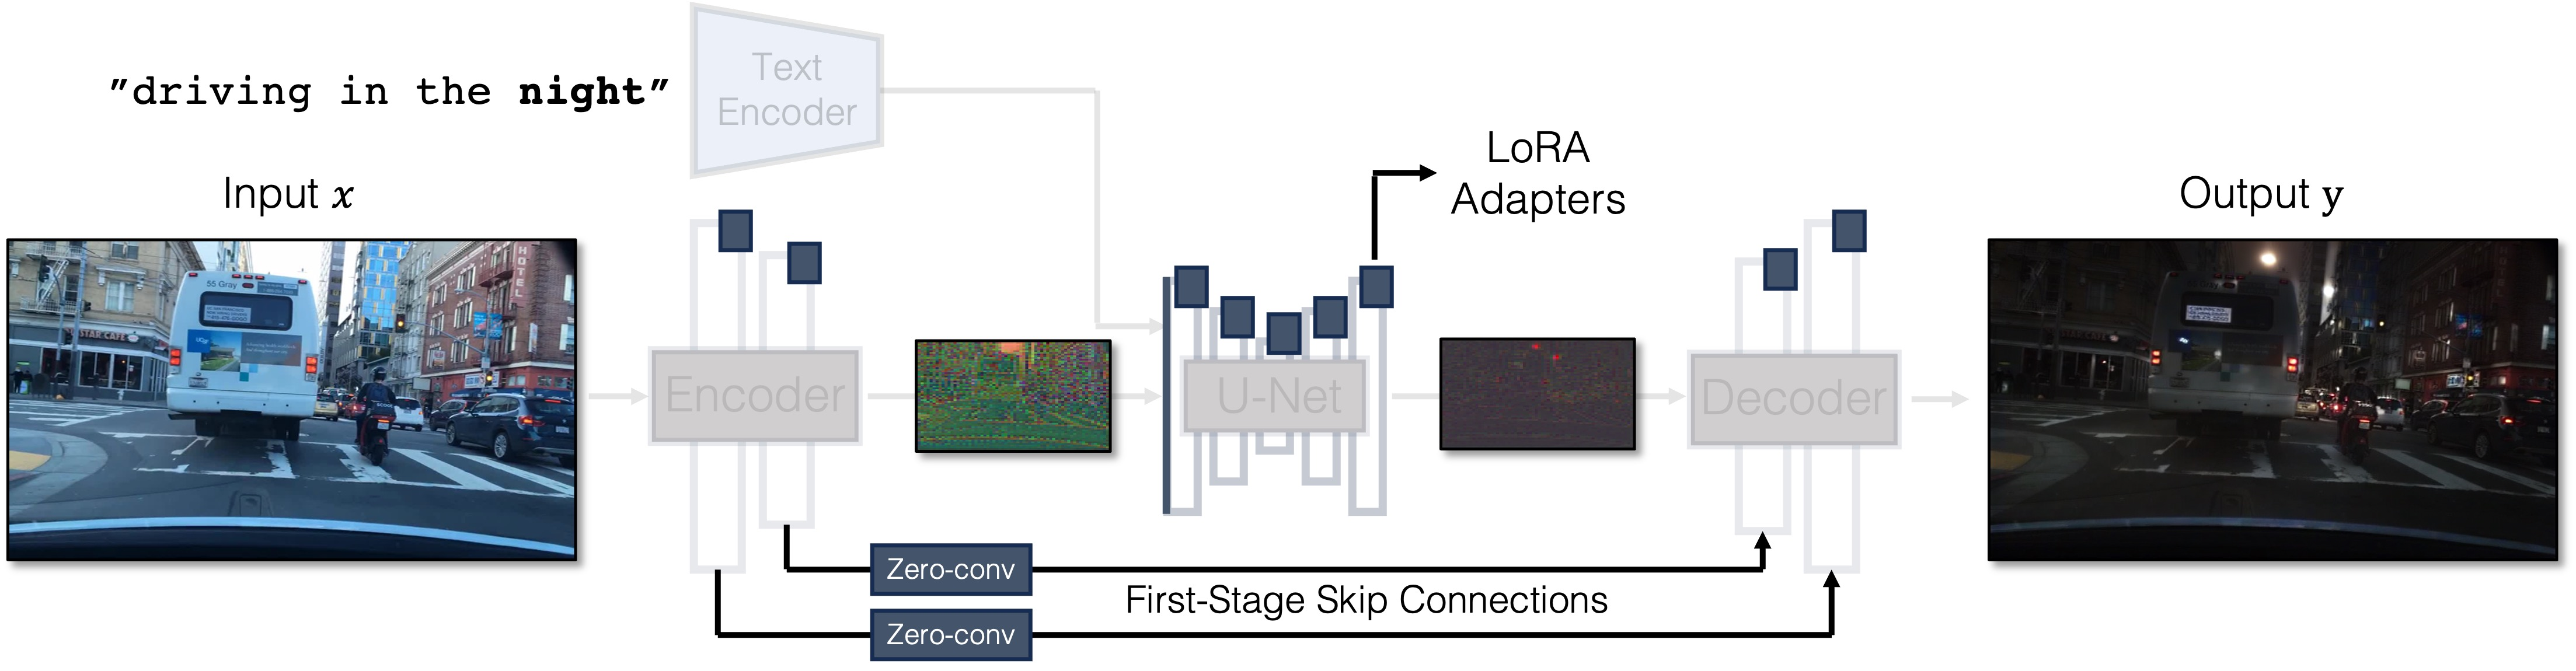
\includegraphics[width=1\linewidth]{images/method.jpg}
    \caption{Model Architecture}
\end{figure}
\end{frame}

% ---------- Unpaired Training ----------
\begin{frame}
    \frametitle{Method}
    \framesubtitle{Unpaired Training}
    \begin{align*}
    \text{Goal:} &\text{ Convert images from } \mathcal{X} \subset \mathbb{R} ^{H \times W \times 3} \
    \text{ to } \mathcal{Y} \subset \mathbb{R} ^{H \times W \times 3} \\
    &\text{ given an unpaired dataset } \mathcal{X} = {x \in \mathcal{X} } \text{ and } \mathcal{Y} = {y \in \mathcal{Y} } \\
    &\text{ using one network } G \text{ and two translations } G(x, c_y): \mathcal{X} \rightarrow \mathcal{Y} \
    \text{ and } G(y, c_x): \mathcal{Y} \rightarrow \mathcal{X}
    \end{align*}
    \end{frame}

\begin{frame}
\frametitle{Method}
\framesubtitle{Unpaired Training}
\begin{block}{Cycle consistency with perceptual loss}
    \begin{equation}
        \mathcal{L}_{\text{cycle}}(G, F) = \mathbb{E}_x [ \mathcal{L}_\text{rec} (G(G(x,c_Y), c_X), x) ] + \mathbb{E}_y [ \mathcal{L}_\text{rec} (G(G(y,c_X), c_Y), y) ]
    \end{equation}
\end{block}
with $\mathcal{L}_{\text{rec}}$ as combination of L1 and LPIPS \cite{zhang2018unreasonable}
\begin{block}{Adversarial loss}
    \begin{align}
        \mathcal{L}_{\text{GAN}} &= \mathbb{E}_{y} [\log D_Y(y)] + \mathbb{E}_{x} [\log(1 - D_Y(G(x,c_Y)))] \\
        &+ \mathbb{E}_{x} [\log D_X(x)] + \mathbb{E}_{Y} [\log(1 - D_X(G(y,c_X)))]
    \end{align}
\end{block}
\end{frame}

\begin{frame}
\frametitle{Method}
\framesubtitle{Unpaired Training}
\begin{block}{Identity regularization loss}
    \begin{equation}
        \mathcal{L} _{\text{idt}} = \mathbb{E} _y [ \mathcal{L}_{\text{rec}}(G(y,c_Y),y)] + \mathbb{E}_x [ \mathcal{L}_{\text{rec}}(G(x,c_X),x)]
    \end{equation}
\end{block}

\begin{block}{Full objective}
    \begin{equation}
        \arg \underset{G}{\min} \mathcal{L}_{\text{cycle}} + \lambda _{\text{idt}} \mathcal{L}_{\text{idt}} + \lambda_{\text{GAN}}\mathcal{L}_{\text{GAN}}
    \end{equation}
\end{block}
    

\end{frame}


% ---------- Extensions ----------
\begin{frame}
\frametitle{Method}
\framesubtitle{Extensions - Paired Training}
\begin{itemize}
    \item Adaptation of network G to paired setting, like edge-to-image or sketch-to-image, called pix2pix-Turbo
    \item new translation function $G(x,c): X \rightarrow Y$ where $X$ is source domain, $Y$ target domain and $c$ conditioning input
\end{itemize}
\begin{block}{Loss Function}
    \begin{equation}
        \arg \underset{G}{\min} \mathcal{L}_{\text{rec}}+ \lambda _{\text{clip}}\mathcal{L}_{\text{CLIP}}+ \lambda_{\text{GAN}}\mathcal{L}_{\text{GAN}}
    \end{equation}
\end{block}
\end{frame}

\begin{frame}
    \frametitle{Method}
    \framesubtitle{Extensions - Generating diverse output}
    Introduction of interpolation coefficient $\gamma$ \newline 
    Three changes to the Architecture (1/3):
    \begin {itemize}
        \item Generator function $G(x,z,\gamma)$ combines noise z and encoder output like so: $\gamma G_{\text{enc}}(x) + (1 - \gamma) z$
        \item Output as U-Net input
    \end{itemize}
\end{frame}

\begin{frame}
    \frametitle{Method}
    \framesubtitle{Extensions - Generating diverse output}
    Three changes to the Architecture (2/3):
    \begin {itemize}
        \item Scale LoRA weights and skip connections according to $\theta = \theta_0 + \gamma \Delta \theta$  
        \item where $\theta_0$ and $\Delta \theta$ denote the original weights and new weights.
    \end{itemize}
\end{frame}

\begin{frame}
    \frametitle{Method}
    \framesubtitle{Extensions - Generating diverse output}
    Three changes to the Architecture (3/3):
    \begin {itemize}
        \item Scale reconstruction loss according to $\gamma$: $\mathcal{L}_{\text{diverse}} = \mathcal{L}_{x,y,z,\gamma} \gamma\mathcal{L}_{\text{rec}}(G(x,z,\gamma),y)]$
        \item $\gamma = 0$ corresponds to default stochastic behavior of pretrained model, in this cas reconstruction loss is not enforced
        \item $\gamma = 1$ corresponds to deterministic translation from previoues seections
    \end{itemize}
\end{frame}
